%%%%%%%%%%%%%%%%%%%%%%%%%%%%%%%%%%%%%%%%%
% Programming/Coding Assignment
% LaTeX Template
%
% This template has been downloaded from:
% http://www.latextemplates.com
%
% Original author:
% Ted Pavlic (http://www.tedpavlic.com)
%
% Note:
% The \lipsum[#] commands throughout this template generate dummy text
% to fill the template out. These commands should all be removed when 
% writing assignment content.
%
% This template uses a Perl script as an example snippet of code, most other
% languages are also usable. Configure them in the "CODE INCLUSION 
% CONFIGURATION" section.
%
%%%%%%%%%%%%%%%%%%%%%%%%%%%%%%%%%%%%%%%%%

%----------------------------------------------------------------------------------------
%	PACKAGES AND OTHER DOCUMENT CONFIGURATIONS
%----------------------------------------------------------------------------------------

\documentclass{article}
%\documentclass[11pt]{article}
\usepackage{fancyhdr} % Required for custom headers
\usepackage{lastpage} % Required to determine the last page for the footer
\usepackage{extramarks} % Required for headers and footers
\usepackage[usenames,dvipsnames]{color} % Required for custom colors
\usepackage{graphicx} % Required to insert images
\usepackage{subcaption}
\usepackage{listings} % Required for insertion of code
\usepackage{courier} % Required for the courier font
\usepackage{amsmath}
\usepackage{framed}

% Margins
\topmargin=-0.45in
\evensidemargin=0in
\oddsidemargin=0in
\textwidth=6.5in
\textheight=9.0in
\headsep=0.25in

\linespread{1.1} % Line spacing

% Set up the header and footer
\pagestyle{fancy}
\lhead{\hmwkAuthorName} % Top left header
\chead{\hmwkClass\ (\hmwkClassTime): \hmwkTitle} % Top center head
%\rhead{\firstxmark} % Top right header
\lfoot{\lastxmark} % Bottom left footer
\cfoot{} % Bottom center footer
\rfoot{Page\ \thepage\ of\ \protect\pageref{LastPage}} % Bottom right footer
\renewcommand\headrulewidth{0.4pt} % Size of the header rule
\renewcommand\footrulewidth{0.4pt} % Size of the footer rule

\setlength\parindent{0pt} % Removes all indentation from paragraphs

%----------------------------------------------------------------------------------------
%	CODE INCLUSION CONFIGURATION
%----------------------------------------------------------------------------------------

\definecolor{mygreen}{rgb}{0,0.6,0}
\definecolor{mygray}{rgb}{0.5,0.5,0.5}
\definecolor{mymauve}{rgb}{0.58,0,0.82}

\lstset{ %
  backgroundcolor=\color{white},   % choose the background color
  basicstyle=\footnotesize,        % size of fonts used for the code
  breaklines=true,                 % automatic line breaking only at whitespace
  captionpos=b,                    % sets the caption-position to bottom
  commentstyle=\color{mygreen},    % comment style
  escapeinside={\%*}{*)},          % if you want to add LaTeX within your code
  keywordstyle=\color{blue},       % keyword style
  stringstyle=\color{mymauve},     % string literal style
}

%----------------------------------------------------------------------------------------
%	DOCUMENT STRUCTURE COMMANDS
%	Skip this unless you know what you're doing
%----------------------------------------------------------------------------------------

% Header and footer for when a page split occurs within a problem environment
\newcommand{\enterProblemHeader}[1]{
%\nobreak\extramarks{#1}{#1 continued on next page\ldots}\nobreak
%\nobreak\extramarks{#1 (continued)}{#1 continued on next page\ldots}\nobreak
}

% Header and footer for when a page split occurs between problem environments
\newcommand{\exitProblemHeader}[1]{
%\nobreak\extramarks{#1 (continued)}{#1 continued on next page\ldots}\nobreak
%\nobreak\extramarks{#1}{}\nobreak
}

\setcounter{secnumdepth}{0} % Removes default section numbers
\newcounter{homeworkProblemCounter} % Creates a counter to keep track of the number of problems
\setcounter{homeworkProblemCounter}{0}

\newcommand{\homeworkProblemName}{}
\newenvironment{homeworkProblem}[1][Problem \arabic{homeworkProblemCounter}]{ % Makes a new environment called homeworkProblem which takes 1 argument (custom name) but the default is "Problem #"
\stepcounter{homeworkProblemCounter} % Increase counter for number of problems
\renewcommand{\homeworkProblemName}{#1} % Assign \homeworkProblemName the name of the problem
\section{\homeworkProblemName} % Make a section in the document with the custom problem count
\enterProblemHeader{\homeworkProblemName} % Header and footer within the environment
}{
\exitProblemHeader{\homeworkProblemName} % Header and footer after the environment
}

\newcommand{\problemAnswer}[1]{ % Defines the problem answer command with the content as the only argument
\noindent\framebox[\columnwidth][c]{\begin{minipage}{0.98\columnwidth}#1\end{minipage}} % Makes the box around the problem answer and puts the content inside
}

\newcommand{\homeworkSectionName}{}
\newenvironment{homeworkSection}[1]{ % New environment for sections within homework problems, takes 1 argument - the name of the section
\renewcommand{\homeworkSectionName}{#1} % Assign \homeworkSectionName to the name of the section from the environment argument
\subsection{\homeworkSectionName} % Make a subsection with the custom name of the subsection
\enterProblemHeader{\homeworkProblemName\ [\homeworkSectionName]} % Header and footer within the environment
}{
\enterProblemHeader{\homeworkProblemName} % Header and footer after the environment
}

%----------------------------------------------------------------------------------------
%	NAME AND CLASS SECTION
%----------------------------------------------------------------------------------------

\newcommand{\hmwkTitle}{Problem Set 2} % Assignment title
\newcommand{\hmwkDueDate}{Sunday, Nov 4\textsuperscript{th}, 2018} % Due date
\newcommand{\hmwkClass}{CSC458} % Course/class
\newcommand{\hmwkClassTime}{LEC 5101} % Class/lecture time
\newcommand{\hmwkAuthorName}{Zhongtian Ouyang} % Your name
\newcommand{\hmwkAuthorID}{1002341012} % Your name

%----------------------------------------------------------------------------------------
%	TITLE PAGE
%----------------------------------------------------------------------------------------

\title{
\vspace{2in}
\textmd{\textbf{\hmwkClass:\ \hmwkTitle}}\\
\normalsize\vspace{0.1in}\small{Due\ on\ \hmwkDueDate}\\
\vspace{0.1in}
\vspace{3in}
}

\author{\textbf{\hmwkAuthorName}\\ \textbf{\hmwkAuthorID}}

\date{} % Insert date here if you want it to appear below your name

%----------------------------------------------------------------------------------------\
\begin{document}

\maketitle
\clearpage

%----------------------------------------------------------------------------------------
%	Common Tools
%----------------------------------------------------------------------------------------
%\begin{framed}
%\begin{lstlisting}[language=matlab]
%\end{lstlisting}
%\end{framed}

%\begin{figure}[h!]
%\centering
%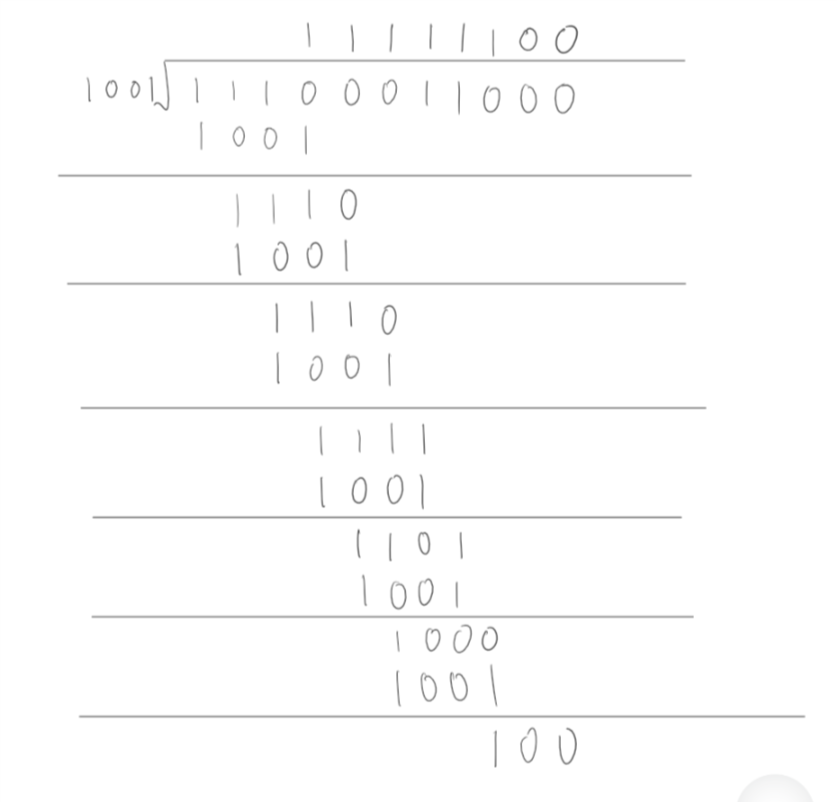
\includegraphics[width=0.6\linewidth]{q10a.png}
%\label{fig:q10a}
%\end{figure}\\
%----------------------------------------------------------------------------------------
%	PROBLEM 1
%----------------------------------------------------------------------------------------

% To have just one problem per page, simply put a \clearpage after each problem
\begin{homeworkProblem}

\noindent \textit{BGP}\\

a)\\
There are three routes to P Provider Q's BGP could receive. P can be arrived from Q through links {1, 2, 3}\\

b)\\
From B to A, Provider P will choose to use link 1. From A to B, Provider Q will choose to use link 2.

\end{homeworkProblem}
%----------------------------------------------------------------------------------------
%	PROBLEM 2
%----------------------------------------------------------------------------------------

\begin{homeworkProblem}
\noindent \textit{IP}\\

a)\\
For inbound traffic, all trafic need to be first send to the entry point IP address the organization holds, which corresponds to an specific address, the address of the headquarter, for example. And then send to the actual destination through the organization's own links. All the traffic enters the organization at a single point. This could be inefficient because the organization is international. The geographical address of the actual destination could be far away from the IP address's geographical address. There could be alternative shorter paths from source to destination.\\

b)\\
The organization can have its own routing table, which contains information about which destination ip correspond to which geographical location. When there is an outbound traffic, it could route the traffic to the exit point geographically closest to the destination.\\

c)\\
The organization should divide its internal network to several subnets base on geographical location. For example, the servers in USA share a subnet while servers in Asia share another. The routers in outside world could then add seperate routing entries for each subnet.\\

d)\\
The internal routers need to be able to recognize internal destinations and have entries to all the other internal networks using internal routes.  
\end{homeworkProblem}
%----------------------------------------------------------------------------------------
%	PROBLEM 3
%----------------------------------------------------------------------------------------

\begin{homeworkProblem}
\noindent \textit{Sequence Number}\\

When setting up an TCP connection, the ISN(initial sequence number) is set to an random number between 0 and $2^{32} - 1$ for reasons discussed in lecture. Therefore, if the ISN is a very large number close to $2^{32} - 1$,  without wrap around, the sequence number runs out quickly after a few packets.
\end{homeworkProblem}
\clearpage
%----------------------------------------------------------------------------------------
%	PROBLEM 4
%----------------------------------------------------------------------------------------

\begin{homeworkProblem}
\noindent \textit{Fast retransmit}\\

Suppose the segment S0 is sent at t = 0. With lossless connection, S7 is sent at t = 700; ACK for S0 should arrive at t = 800, so the packet S8 can be sent at t = 800.\\
Now with a loss of S0, we can't send S8 at t = 800 because the window size is 8. We received the three duplicate ACKs at t = 900, 1000, 1100. With fast retransmit, S0 is retransmitted at t = 1100, ACK of S0 is received at t = 1900. The packet S8 can be sent at t = 1900\\
time lost = 1900 - 800 = 1100ms
\end{homeworkProblem}
%----------------------------------------------------------------------------------------
%	PROBLEM 5
%----------------------------------------------------------------------------------------
\begin{homeworkProblem}
\noindent \textit{TCP slow-start}\\
 
Since the client hosts are connect directly to our routers, we can examine the headers of all the tcp packets. Then, we can determine the congestion window from the outbound tcp packet's sequence number and inbound tcp packet's ACK. And by observing the congestion window, we can determine whether the client is using slowstart. \\
For example, when the tcp connection first established, we should observe the sequence number is only one MSS more than the ACK number, aka the congestion window size is 1 MSS.\\
 Also, after a segment with the same sequence number is retransmitted, we should observe the congestion window decreased at least by half. If the three duplicated ACKs is observed, the  congestion window should be decreased by half. If not, then there is a timeout, the congestion window should be reduced to a very small number such as one.

\end{homeworkProblem}

%----------------------------------------------------------------------------------------
%	PROBLEM 6
%----------------------------------------------------------------------------------------
\begin{homeworkProblem}
\noindent \textit{Congestion}\\

The only time the traffic will pass through R1 is when Hs on the left side of R1 communicate with Hs on the right side of R1. Since all links are full-duplex, we only need to consider traffic in one direction. And since the graph is symmetrical, left to right is the same as right to left. In the worst case, the maximum throughput from left side to the right side is 4 * 1 MBps = 4 MBps, which is the capacity of the links of R1. So R1 can not be congested.\\
For all other routers, the router would be congested if all its parent's bandwidth are going toward one of its children, for example, right child. It would be even worse if the left child also send traffic toward right child. The situation is shown in following graph. R3-B link need a bandwidth of 3x but only got a capacity of x.
\begin{figure}[h!]
\centering
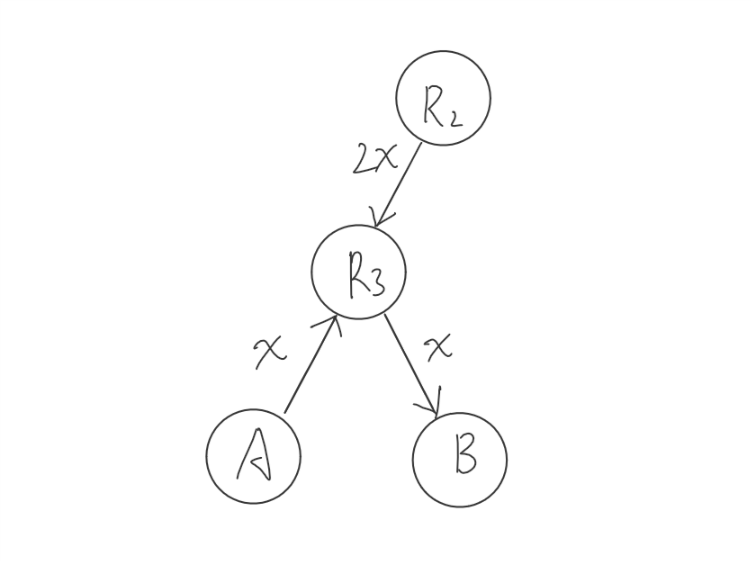
\includegraphics[width=0.37\linewidth]{q6.png}
\label{fig:q10a}
\end{figure}
\end{homeworkProblem}
\clearpage
%----------------------------------------------------------------------------------------
%	PROBLEM 7
%----------------------------------------------------------------------------------------
\begin{homeworkProblem}
\noindent \textit{TCP Ports}\\

a)
$A \rightarrow S$: Source Port: 12345  Destination Port: 23\\

b)
$B \rightarrow S$: Source Port: 23456  Destination Port: 23\\

c)
$S \rightarrow A$: Source Port: 23  Destination Port: 12345\\

d)
$S \rightarrow B$: Source Port: 23  Destination Port: 23456\\

e)\\
Yes. Because A and B are different hosts, the source port from A and source port from B are irrelavant.\\

f)\\
No. Since the are the same host, they have the same ip address. The post number must be different in order to identity difference processes and make sure the information is received by the correct process.


\end{homeworkProblem}
%----------------------------------------------------------------------------------------
%	PROBLEM 8
%----------------------------------------------------------------------------------------
\begin{homeworkProblem}
\noindent \textit{Checksum}\\

Calculate 1's complement sums:\\
01010011 + 01100110 = 10111001, no over flow\\
10111001 + 01110100 = 100101101, 001011101 + 1 = 00101110\\
The checksum is the sum's 1's complement, which is 11010001.\\
We use one's complement of the sum as the checksum because by adding one's complement of the sum to the sum, we got all 1's. It is more efficient to check whether there is an 0 than comparing two numbers and determine whether they are the same.\\
The receiver add the three numbers and checksum together. If no error, the sum should be all 1's. If there is 0 in the sum, there is an error.\\
All 1-bit error will be detected, but 2-bit error can go undetected. For example, if the first two words become 01010010 and 01100111, the sum is unchanged.

\end{homeworkProblem}
%----------------------------------------------------------------------------------------
%	PROBLEM 9
%----------------------------------------------------------------------------------------
\begin{homeworkProblem}
\noindent \textit{AIMD congestion control}

a)\\
Since we increase 1 MSS everytime we received a batch of ACKs, with no loss, we need to receive 6 batches of ACKs to increase cwnd from 6 MSS to 12 MSS. We receive a batch of ACK every 1 RTT. So we need 6 RTT to increase cwnd from 6 MSS to 12 MSS.\\

b)\\
Total MSS sent = 6 + 7 + 8 + 9 + 10 + 11 = 51\\
Average Throughput = 51 MSS / 6 RTT = 8.5 MSS/RTT\\

\end{homeworkProblem}
\clearpage
%----------------------------------------------------------------------------------------
%	PROBLEM 10
%----------------------------------------------------------------------------------------
\begin{homeworkProblem}
\noindent \textit{BGP}\\

a) Router 3c learns about the x from eBGP\\

b) Router 3a learns about the x from iBGP\\

c) Router 1c learns about the x from eBGP\\

d) Router 1d learns about the x from iBGP\\

\end{homeworkProblem}
%----------------------------------------------------------------------------------------
%	PROBLEM 11
%----------------------------------------------------------------------------------------
\begin{homeworkProblem}
\noindent \textit{Dijkstra}\\

\begin{center}
\begin{tabular}{ |c|c|c|c|c|c|c|c| } 
\hline
Steps & S & D(t), p & D(u), p & D(v), p & D(w), p & D(y), p & D(z), p\\ 
\hline
0 & \{x\} & inf, null & inf, null & 3, x & 6, x & 6, x & 8, x\\
1 & \{x, v\} & 7, v & 6, v & 3, x & 6, x & 6, x & 8, x\\
2 & \{x, v, w\}& 7, v & 6, v & 3, x & 6, x & 6, x & 8, x\\
3 & \{x, v, w, y\} & 7, v & 6, v & 3, x & 6, x & 6, x & 8, x\\
4 & \{x, v, w, y, u\} & 7, v & 6, v & 3, x & 6, x & 6, x & 8, x\\
5 & \{x, v, w, y, u, t\} & 7, v & 6, v & 3, x & 6, x & 6, x & 8, x\\
6 & \{x, v, w, y, u, t, z\} & 7, v & 6, v & 3, x & 6, x & 6, x & 8, x\\
\hline
\end{tabular}
\end{center}

Shortest paths:\\
$x \rightarrow t$ : x, v, t\\
$x \rightarrow u$ : x, v, u\\
$x \rightarrow v$ : x, v\\
$x \rightarrow w$ : x, w\\
$x \rightarrow y$ : x, y\\
$x \rightarrow z$ : x, z\\
\end{homeworkProblem}
%----------------------------------------------------------------------------------------
%	PROBLEM 12
%----------------------------------------------------------------------------------------
\begin{homeworkProblem}
\noindent \textit{Sequence Number}\\

a)\\
TCP sequence number has a range from 0 to $2^{32} - 1$. So there are $2^{32}$ possible sequence numbers.\\ 
we increase sequence number by 1 every byte.\\
Maximum value of L = $2^{32} = 4294967296$ bytes\\

b)\\
Number of segments = $\lceil 4294967296 / 536 \rceil = \lceil 8012998.68657 \rceil = 8012999$\\
For each segment, 66 bytes of various headers are added before sent out.\\
Total = $4294967296 + 8012999 \times 66 = 4823825230$ bytes = 38590601840 bits\\
$38590601840 / 155000000 = 248.971624774 s \approx 249 s$


\end{homeworkProblem}
\clearpage
%----------------------------------------------------------------------------------------

\end{document}
